\documentclass{deimj}
\usepackage{graphicx}
\usepackage{listings,jlisting}
%\usepackage{latexsym}
%\usepackage{txfonts}
%\usepackage[fleqn]{amsmath}
%\usepackage[psamsfonts]{amssymb}
%\usepackage[deluxe]{otf}

% 印刷位置調整 %
% 必要に応じて値を変更してください.
\hoffset -10mm % <-- 左に 10mm 移動
\voffset -10mm % <-- 上に 10mm 移動


\lstset{%
  language={c},
  basicstyle={\small},%
  identifierstyle={\small},%
  commentstyle={\small\itshape},%
  keywordstyle={\small\bfseries},%
  ndkeywordstyle={\small},%
  stringstyle={\small\ttfamily},
  frame={tb},
  breaklines=true,
  columns=[l]{fullflexible},%
  numbers=left,%
  xrightmargin=0zw,%
  xleftmargin=3zw,%
  numberstyle={\scriptsize},%
  stepnumber=1,
  numbersep=1zw,%
  lineskip=-0.5ex%
}

\newcommand{\AmSLaTeX}{%
 $\mathcal A$\lower.4ex\hbox{$\!\mathcal M\!$}$\mathcal S$-\LaTeX}
\newcommand{\PS}{{\scshape Post\-Script}}
\def\BibTeX{{\rmfamily B\kern-.05em{\scshape i\kern-.025em b}\kern-.08em
 T\kern-.1667em\lower.7ex\hbox{E}\kern-.125em X}}

\papernumber{DEIM Forum 2014 XX-Y}

\jtitle{BabaScript}
\jsubtitle{人の行動をプログラムに組み込むためのプログラミング環境}
\authorlist{%
 \authorentry[bb@sfc.keio.ac.jp]{馬場 匠見}{Takumi BABA}{Keio}% 
 \authorentry[shokai@sfc.keio.ac.jp]{橋本 翔}{Sho HASHIMOTO}{Keio}% 
 \authorentry[masui@pitecan.com]{増井 俊之}{Toshiyuki MASUI}{Keio-Faculty}% 
}
\affiliate[Keio]{慶應義塾大学政策・メディア研究科\hskip1zw
  〒252-0882 神奈川県藤沢市遠藤5322}
 {Graduate School of Media and Governance,
  Keio University\\
  5322 Endo, Fujisawa,
  Kanagawa 252-0882, Japan}
\affiliate[Keio-Faculty]{慶應義塾大学環境情報学部\hskip1zw
  〒252-0882 神奈川県藤沢市遠藤5322}
 {Faculty of Environment and Information Studies,
   Keio University\\
  5322 Endo, Fujisawa,
  Kanagawa 252-8520, Japan}  

%\MailAddress{$\dagger$hanako@deim.ac.jp,
% $\dagger\dagger$\{taro,jiro\}@jforum.co.jp}

\begin{document}
\pagestyle{empty}
\begin{jabstract}
コンピュータの動作の手順書としてプログラムが、人間の行動の手順書としてマニュアルやレシピといったものが存在する。
プログラム上で人の行動を記述するためのプログラミング環境 BabaScript を提案する。
BabaScriptは、人への命令構文と値を返すことのできるクライアントアプリケーションを組み合わせることで、人オブジェクトをプログラム上で表現可能にするための一連の仕組みだ。

\end{jabstract}
\begin{jkeyword}
ヒューマンコンピュテーション, プログラミング環境
\end{jkeyword}
\maketitle

\section{はじめに}

コンピュータの動作を制御するための手順書としてプログラムが存在する。
世界中のコンピュータがインターネットを介して動作している
実世界をプログラミングするために、センサ・アクチュエータを利用するようになっている
プログラムが記述できる処理は増え続けており、プログラムが干渉可能な世界は大きく広がっている。

一方、人間の動作を制御するための手順書としては、レシピであったりマニュアルといったものが存在する。
手順書に従うことによって、人間は適切・効率的に動作し、目的を達成できる。
レシピやマニュアルの中身は、プログラムと同じようなものである。
人に実行させたい処理が記述されており、人は記述内容を自分で解釈し、実行していく。
例えば、料理のレシピには、

\begin{lstlisting}[caption=,label=]
if 鍋が沸騰したら
  パスタを鍋に投入する
\end{lstlisting}
    
というようなプログラムが、小売店の店員マニュアルでは

\begin{lstlisting}[caption=,label=]
if レジに人が並んでいる
  2番レジを開ける
\end{lstlisting}
    
といったプログラムが記述され、実行されている。

プログラムとレシピやマニュアルは、実行手順を表すという意味では同じものであるが、別の存在として認識されている。
しかし、近年のコンピュータと人間の密接な関係を考慮すると、この状況は変化していくべきである。
レシピやマニュアルの中では、コンピュータを扱う命令が書いてあることはよくある
プログラムの中で、計算資源として人間を使うことも提案されている
人とコンピュータ、両方の世界を記述するための統一的なものは存在せず、両者を同じフォーマットのドキュメントとして記述することはできない。

本論文では、人の行動をプログラム内に記述可能にするプログラミング環境 BabaScript を提案する。
人の行動をプログラム内で記述可能にすることで、同一フォーマットのデータ上で人とコンピュータ両方への命令を記述することができる。

\section{BabaScript}

機械と人をプログラム内で完全に同等に扱えるライブラリ BabaScript を開発した。
BabaScriptは、人への命令構文を含んだオブジェクト(以下、人オブジェクト)を宣言可能にするライブラリだ。
通信用のライブラリを含んだクライアントアプリケーションと組み合わせることによって、人への命令とその実行結果の取得を実現する。

\subsection{人への命令構文}
人への命令構文を含んだオブジェクトを宣言し、そのオブジェクトに対してメソッド実行をすることで、メソッドと引数を元に人への命令内容を生成する。
以下のようなプログラムで人への命令を記述する。

% 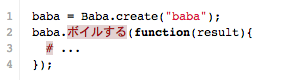
\includegraphics[width=80mm, bb=0 0 300 80]{images/image1.png}
\begin{lstlisting}[caption=,label=]
baba = new Baba.Script("baba");
baba.ボイルする(function(result){
  ...
});
\end{lstlisting}
プログラム側で人オブジェクトを宣言するときには、第一引数にidを指定する。
このidと同一のidを持つクライアントに対し、命令の配信が行われる。
また、複数のクライアントアプリケーションが同一のidによって生成されている場合、scriptからの命令は特別な命令がない場合は、クライアントアプリケーションに分散して配信される。


人への命令メソッドの第一引数にオブジェクトを与えることによってクライアントアプリケーション側にオプションとして情報を送ることができる。
特別なオプションとしてbroadcast が存在する。

\begin{lstlisting}[caption=,label=]
baba.ボイルする({broadcast: 5}, function(result){ ... });
\end{lstlisting}
  

上記のように、オプションに broadcast: num を指定することによって、同じidを持つ全クライアントに対して同様の命令を送信し、 num で指定した数だけ値が返ってきたらコールバック関数を実行することができる。

オプションの例としては返り値の型指定がある。
プログラムへの返り値として様々な型が考えられるが、全ての型を考慮してプログラムを記述することは難しい。
返り値の型を指定することによって、プログラム側で求めている値を人に入力させることが可能だ。
例えば、数値の返り値を求める場合であれば、以下のようなプログラムを書き、クライアントアプリケーション側で数値だけを入力させるインタフェースを表示させることで実現する。

\begin{lstlisting}[caption=,label=]
baba.数値を入力してください({format: "int"}, function(result){ ... });
\end{lstlisting}

人への命令構文を含んだオブジェクトに対してメソッドを実行することによって、
クライアントアプリケーションを組み合わせることで、人
人は命令を処理し、その結果を入力すると、プログラムに自動で値が返る。

\subsection{クライアント}

ワーカー側では、命令を受け取り、値をプログラムに返すためのクライアントオブジェクトを生成する。
このクライアントオブジェクトからのメッセージを受け取る関数を実装することによって、プログラマ側で自由にクライアントアプリケーションを実装できる。
以下のようなプログラムでプログラムからのメッセージを受け取る。

\begin{lstlisting}[caption=,label=]
client = new Baba.Client("baba");
client.on("get_task", function(order){
  プログラムからメッセージを受け取った時の挙動を記述する
});
\end{lstlisting}

メッセージを受け取る関数内において、ユーザに命令を伝え、処理結果を入力するようなインタフェースを生成してワーカーに提示する。
また、クライアントオブジェクトが持つメソッド returnValue を使うことで、プログラムに処理結果を返すことができる。
以下のようなプログラムが考えられる。

\begin{lstlisting}[caption=,label=]
client.on("get_task", function(result){
  order = new Order(result.key)
  input = new Input(result.format)
  input.on("submit", function(value){
    client.returnValue(value)
  });  
});
\end{lstlisting}
  
  
\subsection{利用の流れ}
本環境では、以下のような流れで利用される

\begin{enumerate}
\item プログラムで人への命令構文を書く
\item ネットワークを介して、適切なBabaScript Clientに命令が配信される
\item BabaScript Client は、命令をユーザに通知する
\item 人が命令を処理する
\item 人は処理結果をBabaScript Clientに入力する
\item 結果をネットワークを介して、プログラムに返す
\item プログラムは、返ってきた値を元に指定された続きの処理を実行する
\end{enumerate}

\subsection{特徴}
\subsubsection{人力をプログラムに溶けこませる}
普通にプログラムを書いている中で、オブジェクトを扱っているのと同じような手法で人オブジェクトを利用可能である。
人オブジェクトのメソッドを実行すれば、普通のオブジェクトと同じように、値が返ってくる。
真の意味で、人と通常のオブジェクトは同じものとなる。

\subsubsection{あらゆるWebアプリに人力処理を組み込む}
クライアントライブラリを読み込み、クライアントオブジェクトを生成するだけで、あらゆるWebアプリ上で人力処理のワーカーになることができる。
拡張性がとても高く、既存のアプリケーションにも組み込むことができる

\subsection{例}
パスタ料理をつくるプログラムを以下に示す

\subsubsection{script側プログラム}
人への命令を記述するプログラムは、以下のようなものが考えられる。

% 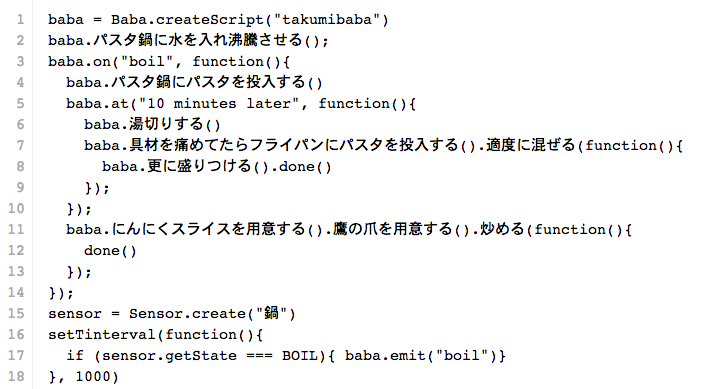
\includegraphics[width=100mm, bb=0 0 713 389]{images/image3.png}
  
\begin{lstlisting}[caption=,label=]
  baba = Baba.createScript("takumibaba")
  baba.パスタ鍋に水を入れ沸騰させる();
  baba.on("boil", function(){
    baba.パスタ鍋にパスタを投入する()
    baba.at("10 minutes later", function(){
      baba.湯切りする()
      baba.具材を痛めてたらフライパンにパスタを投入する().適度に混ぜる(function(){
        baba.更に盛りつける().done()
      });
    });
    baba.にんにくスライスを用意する().鷹の爪を用意する().炒める(function(){
      done()
    });   
  });
  sensor = Sensor.create("鍋")
  setTinterval(function(){
    if (sensor.getState === BOIL){ baba.emit("boil")}
  }, 1000)
\end{lstlisting}
  

\subsubsection{client側プログラム}
人への命令を受け取り、ユーザに提示するプログラムは以下のようなものが考えられる。
% 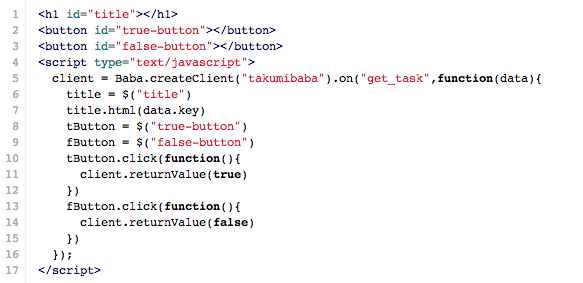
\includegraphics[width=100mm, bb=0 0 583 283]{images/image2.png}

\begin{lstlisting}[caption=,label=]
   <h1 id="title"></h1>
    <button id="true-button"></button>
    <button id="false-button"></button>
    <script type="text/javascript">
      client = Baba.createClient("takumibaba").on("get_task",function(data){
        title = $("title")
        title.html(data.key)
        tButton = $("true-button")
        fButton = $("false-button")
        tButton.click(function(){
          client.returnValue(true)
        })
        fButton.click(function(){
          client.returnValue(false)
        })
      });
    </script>
\end{lstlisting}
    
  
\subsubsection{クライアント}
クライアントアプリは、以下のようなインタフェースを持つ。

\section{関連研究}
計算機では処理できないようなタスクを解決するために、人を計算資源としてプログラムに組み込む手法はヒューマンコンピュテーション\cite{HumanComputation}と呼ばれ、様々な研究が行われている。

米Amazonが運営している Amazon MechaicalTurk\cite{amt} は、クラウドソーシングのためのプラットフォームだ。

AUTOMAN\cite{automan}は、cloudprogrammingという概念を唱え、通常のプログラミング言語内で、コンピュータによる計算と人による計算を統合した。
CrowdForge\cite{crowdforge}は、クラウドソーシングのためのMapReduce実装をした。
クラウドソーシングするタスクを適切に分割し、人力で解かせた後、集合させるためのツールキットだ。
jabbewocky\cite{jabberwocky}は、
CrowdDB\cite{crowddb}では機械だけでは答えられないようなDBへのクエリに対し、クラウドソーシングを使うことで返答させるためのSQLライクなプログラミングを提案している。
CyLog\cite{cylog}は
クラウドソーシング/ヒューマンコンピュテーション系の研究は、人を計算資源として捉え、コンピュータの代替として人に処理を行わせることをやっている。
本研究では、人の行動そのものを記述する。
その中で、コンピュータの代替としての行動を記述することもある。

Human As Sensorなんてものもある。
Using Stanger as Sensorsでは
PRISMでは

\section{おわりに}

\vspace{30mm}

\begin{thebibliography}{99}
\bibitem{humancomputation}
L. von Ahn. 2007. Human computation. In Proceedings of the 4th international conference on Knowledge capture. K-CAP '07. ACM.
\bibitem{amt}
Amazon Machanical Turk
http://www.mturk.com
\bibitem{automan}
\bibitem{crowdforge}
\bibitem{jabberwocky}
\bibitem{crowddb}
\bibitem{cylog}
\end{thebibliography}


\end{document}
